\documentclass[border=10pt]{standalone}
\usepackage{tikz}
\usetikzlibrary{shapes.geometric, arrows.meta, positioning, fit, shadows}

\begin{document}

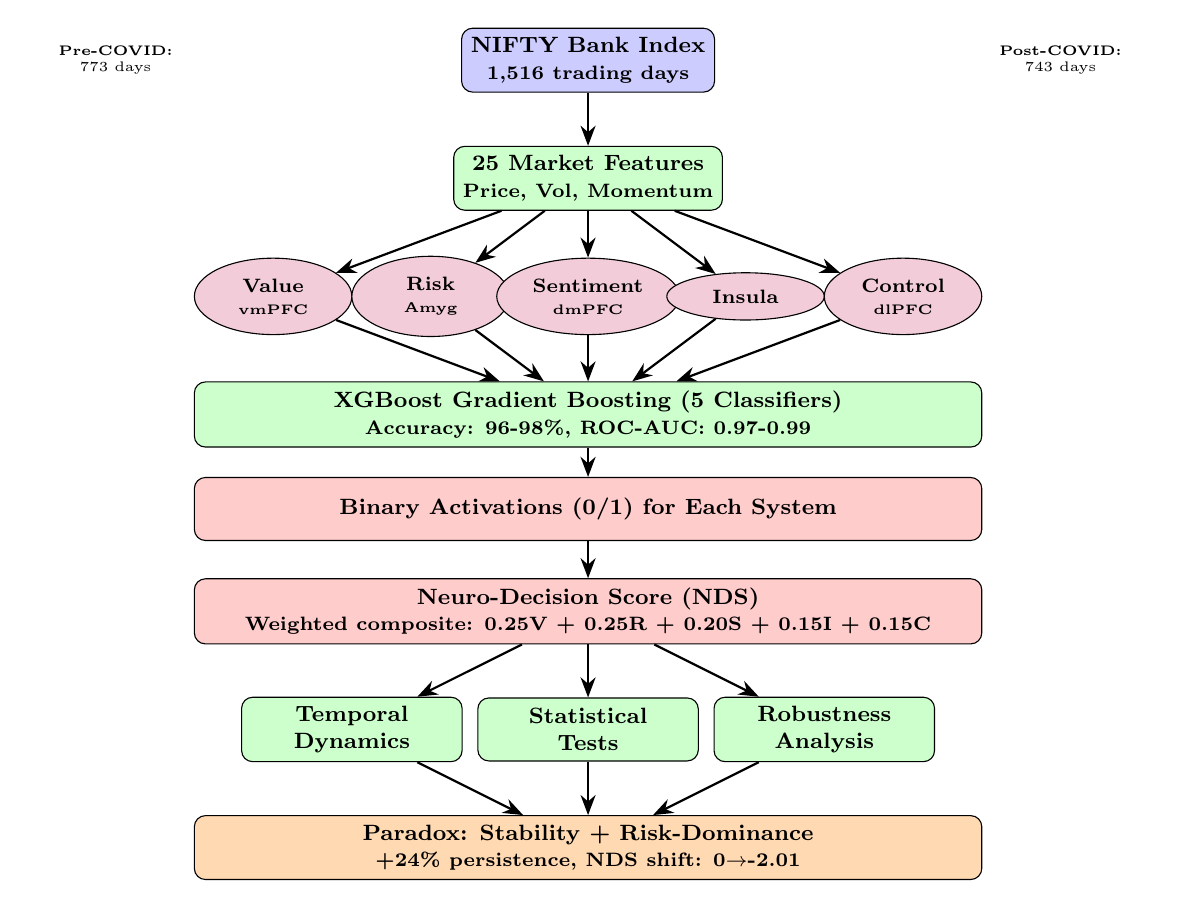
\begin{tikzpicture}[
    node distance=1.2cm,
    every node/.style={align=center},
    data/.style={rectangle, rounded corners, minimum width=2.8cm, minimum height=0.8cm, text centered, draw=black, fill=blue!20, font=\footnotesize\bfseries},
    process/.style={rectangle, rounded corners, minimum width=2.8cm, minimum height=0.8cm, text centered, draw=black, fill=green!20, font=\footnotesize\bfseries},
    brain/.style={ellipse, minimum width=2cm, minimum height=0.6cm, text centered, draw=black, fill=purple!20, font=\scriptsize\bfseries},
    result/.style={rectangle, rounded corners, minimum width=2.8cm, minimum height=0.8cm, text centered, draw=black, fill=red!20, font=\footnotesize\bfseries},
    arrow/.style={-{Stealth[scale=1.1]}, thick}
]

% Layer 1: Input Data
\node[data] (input) at (0, 6) {NIFTY Bank Index\\{\scriptsize 1,516 trading days}};

% Layer 2: Feature Engineering
\node[process] (features) at (0, 4.5) {25 Market Features\\{\scriptsize Price, Vol, Momentum}};

% Layer 3: Five Brain Systems
\node[brain] (value) at (-4, 3) {Value\\{\tiny vmPFC}};
\node[brain] (risk) at (-2, 3) {Risk\\{\tiny Amyg}};
\node[brain] (sentiment) at (0, 3) {Sentiment\\{\tiny dmPFC}};
\node[brain] (insula) at (2, 3) {Insula};
\node[brain] (control) at (4, 3) {Control\\{\tiny dlPFC}};

% Layer 4: XGBoost Classification
\node[process, minimum width=10cm] (xgboost) at (0, 1.5) {XGBoost Gradient Boosting (5 Classifiers)\\{\scriptsize Accuracy: 96-98\%, ROC-AUC: 0.97-0.99}};

% Layer 5: Activations
\node[result, minimum width=10cm] (activations) at (0, 0.3) {Binary Activations (0/1) for Each System};

% Layer 6: NDS
\node[result, minimum width=10cm] (nds) at (0, -1) {Neuro-Decision Score (NDS)\\{\scriptsize Weighted composite: 0.25V + 0.25R + 0.20S + 0.15I + 0.15C}};

% Layer 7: Analysis
\node[process] (temporal) at (-3, -2.5) {Temporal\\Dynamics};
\node[process] (stats) at (0, -2.5) {Statistical\\Tests};
\node[process] (robust) at (3, -2.5) {Robustness\\Analysis};

% Layer 8: Results
\node[result, minimum width=10cm, fill=orange!30] (results) at (0, -4) {\textbf{Paradox: Stability + Risk-Dominance}\\{\scriptsize +24\% persistence, NDS shift: 0$\rightarrow$-2.01}};

% Arrows
\draw[arrow] (input) -- (features);
\draw[arrow] (features) -- (value);
\draw[arrow] (features) -- (risk);
\draw[arrow] (features) -- (sentiment);
\draw[arrow] (features) -- (insula);
\draw[arrow] (features) -- (control);
\draw[arrow] (value) -- (xgboost);
\draw[arrow] (risk) -- (xgboost);
\draw[arrow] (sentiment) -- (xgboost);
\draw[arrow] (insula) -- (xgboost);
\draw[arrow] (control) -- (xgboost);
\draw[arrow] (xgboost) -- (activations);
\draw[arrow] (activations) -- (nds);
\draw[arrow] (nds) -- (temporal);
\draw[arrow] (nds) -- (stats);
\draw[arrow] (nds) -- (robust);
\draw[arrow] (temporal) -- (results);
\draw[arrow] (stats) -- (results);
\draw[arrow] (robust) -- (results);

% Period labels
\node[font=\tiny, text width=2cm] at (-6, 6) {\textbf{Pre-COVID:}\\773 days};
\node[font=\tiny, text width=2cm] at (6, 6) {\textbf{Post-COVID:}\\743 days};

\end{tikzpicture}

\end{document}
